\section{Description générale du modèle}

\subsection{Cas d'utilisation}
Voici le diagramme des cas d'utilisation que nous avons choisi et qui définira par la suite certaines contraintes de notre modèle :\\

\begin{figure}[H]
  \center
  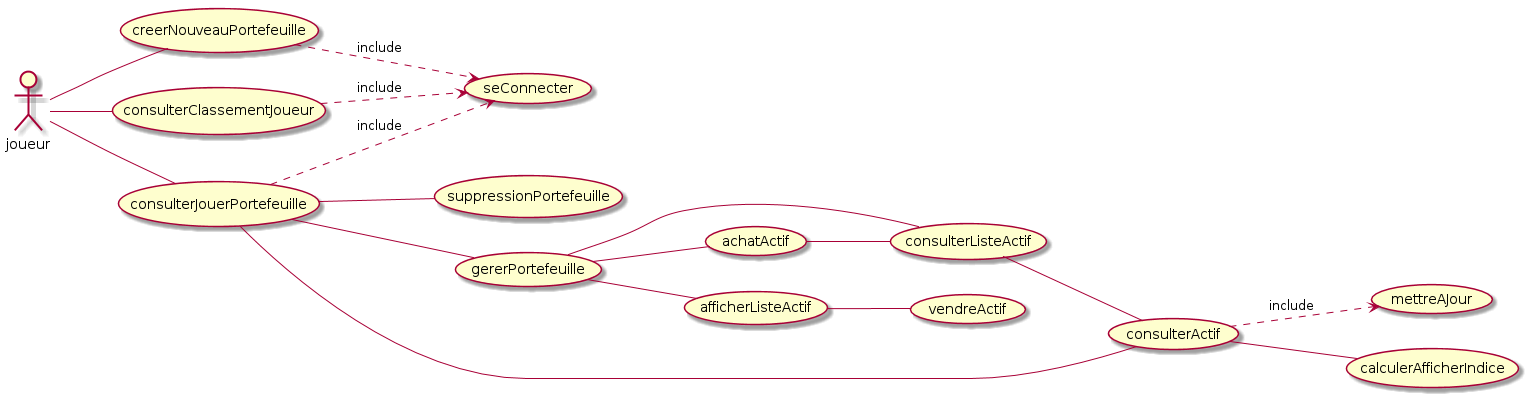
\includegraphics[scale=0.35]{../graph/CasDutilisationGeneral.png} 
\end{figure}

Un joueur peut : créer un nouveau portefeuille, consulter l'état du jeu (i.e. le classement des joueurs) ou encore consulter et jouer avec son portefeuille, sous réserve qu'il se soit connecté au préalable. \\ \\
Lorsqu'il choisit de consulter et jouer avec son portefeuille, quatre options s'offrent à lui : il peut consulter un actif précis, consulter la liste des actifs côtés s'il ne sait pas exactement ce qu'il cherche, gérer son portefeuille et jouer, ou encore supprimer son portefeuille afin de stopper la partie. \\ \\
Si le joueur consulte un actif, la bourse sera mise à jour avant qu'il ne puisse éventuellement récupérer un indicateur technique sur ce titre.\\ \\
Si le joueur consulte la liste des actifs, il pourra alors en sélectionner un et se retrouvera dans le cas précédent. \\ \\
Si le joueur choisit de gérer son portefeuille, il peut consulter la liste des actifs de la bourse (et se retrouvera dans la situation précédente), il peut aussi acheter un actif en parcourant la bourse (liste des actifs), et sa dernière possibilité consiste en la consultation des actifs présents dans son portefeuille avant de pouvoir, s'il le souhaite, en vendre une partie.
